\documentclass{article}

\usepackage[utf8]{inputenc}
\usepackage[english]{babel}
\usepackage{a4}
\usepackage[T1]{fontenc}
\usepackage[cyr]{aeguill}
\usepackage{graphicx}
\usepackage{amsmath}
\usepackage{authblk}
\usepackage{listings}
\usepackage{subfigure}
\usepackage{float}
\usepackage{geometry}
\usepackage[a4paper]{geometry} % Marges plus larges
\geometry{hmargin=2.5cm,vmargin=1.65cm}
\usepackage[sectionbib]{chapterbib}



\title{TS114 Signal processing \\ MICA Project}



\author{ABIED Imad \\ Email: imad.abied@bordeaux-inp.fr

\and AHALLI Mohamed \\ Email: mohamed.ahalli@bordeaux-inp.fr

\and BIGI Mohamed \\ Email:  mohamed.bigi@bordeaux-inp.fr }

\date{11/05/2021}

                 
\sloppy      

\begin{document}
\maketitle
\begin{center}
    ENSEIRB-MATMECA
\end{center}

\tableofcontents

\newpage

\section{Introduction}

The goal of this project was to analyse signals obtained from measuring heart electrical activity. Such a signal is called electrocardiogram, ECG for short.
ECG respects the pattern described in figure 1. Detecting this pattern consists of identifying the four characteristic points P, Q, R,S and T in each R-R interval from a real ECG signal, as shown in figure 2. The algorithm for this task is presented in the technical part below.

\begin{figure}[htbp]

\centerline{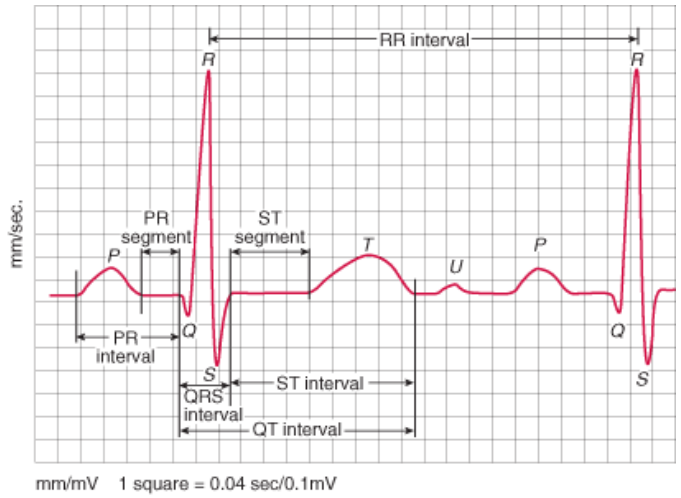
\includegraphics[scale = 0.5]{figure_1.png}}
\caption{ECG pattern}

\centerline{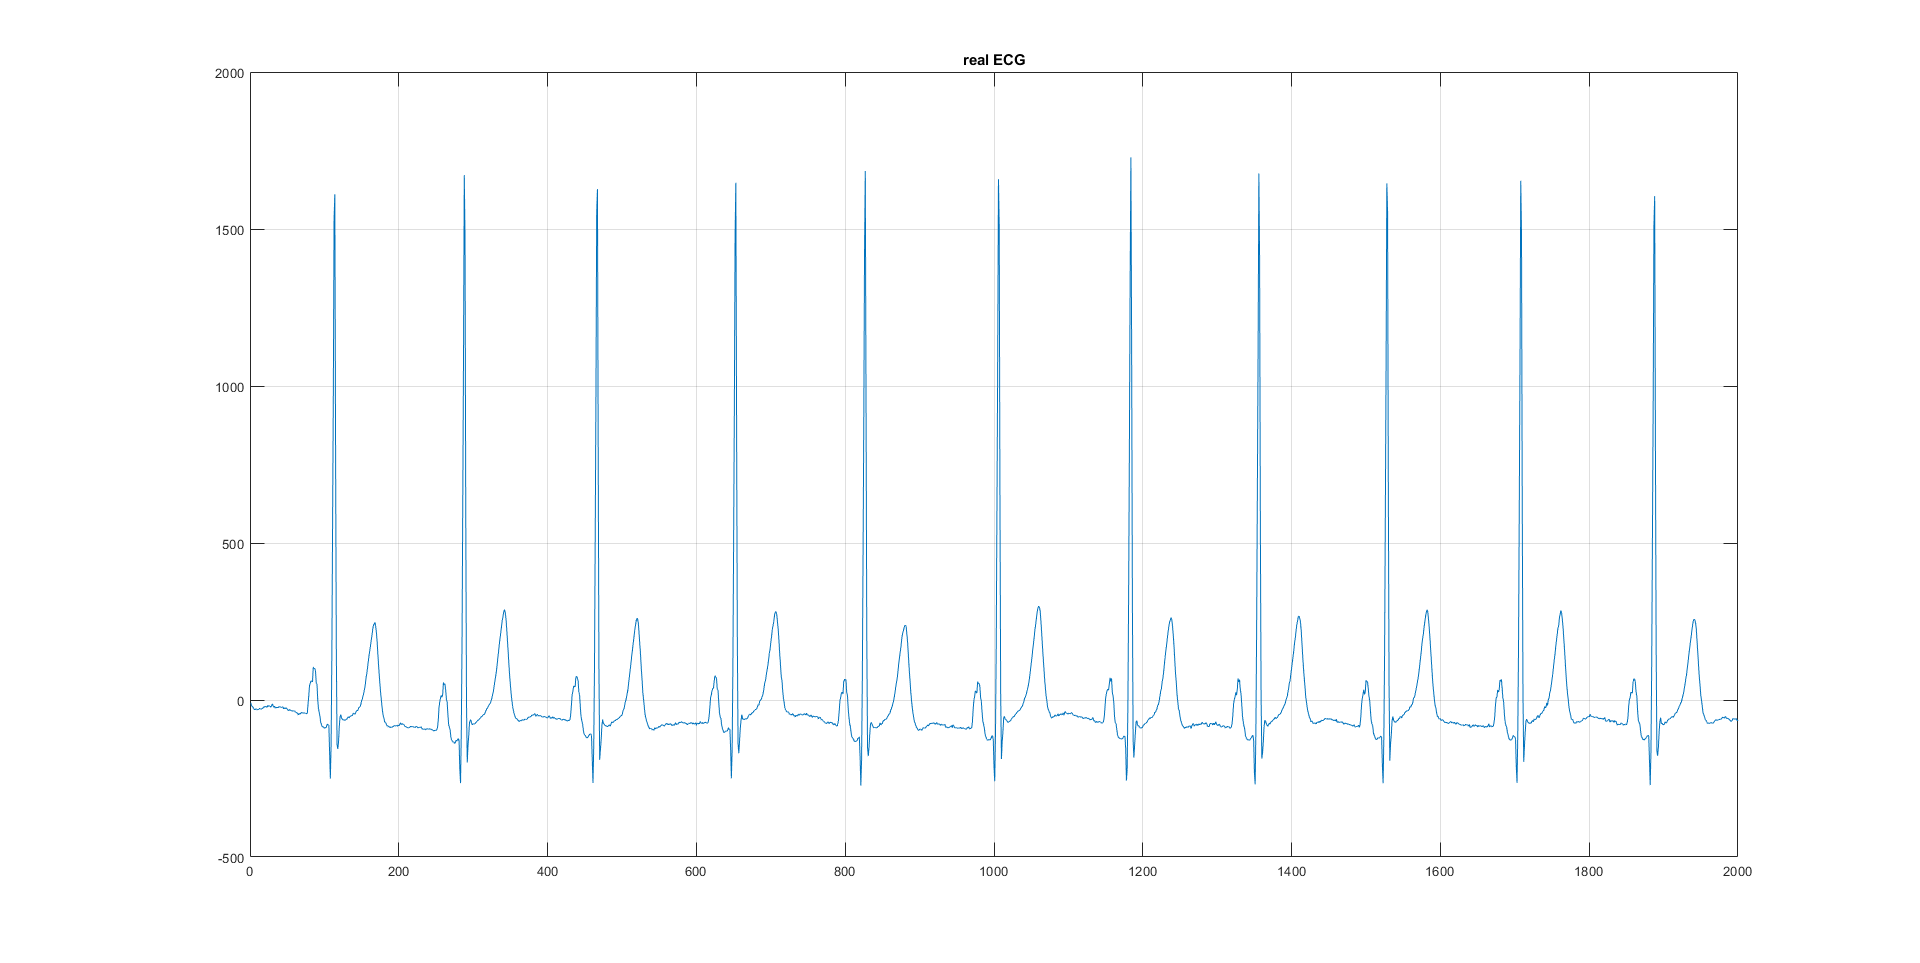
\includegraphics[scale = 0.3]{figure_2.png}}
\caption{Real ECG signal}

\end{figure}

Furthermore, cardiac pathologies are defined from the PQRST mathematical properties. Therefore, the identification of cardiac pathologies can be automatic. Algorithms for automatic identification are discussed in the technical part of this report.

PQRST mathematical properties can change over time for different reasons. For example, the heart rate increases after doing a physical activity. This is why the spectrogram was used during the project. The spectrogram was employed to understand how ECG characteristics change in the course of time, enabling us to choose the right time interval to apply desired algorithms. For that reason the first section of the technical part is dedicated to spectrograms.

\section{Data visualization (spectrogram) }
Spectrograms are used to locally represent the spectrum of a signal. As the spectrum is a statistical measurement, it’s necessary to define the term “locally” by a window of a certain length noted N. The larger the window, the greater frequency precision is obtained at the price of losing time accuracy. Conversely, The shorter window, the greater time accuracy is obtained at the cost of losing frequency precision. This is because there is more data to process in order to establish the spectre, which is a statistical measure. Nevertheless, the spectrum computed by a large window is not “very local".

\begin{figure}[H]

\begin{subfigure}

\centerline{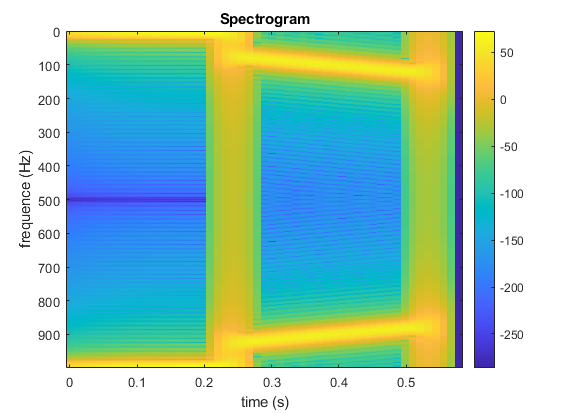
\includegraphics[scale = 0.6]{figure_3_large_window.png}}
\caption{Spectrogram with a large window.}
\end{subfigure}

\begin{subfigure}

\centerline{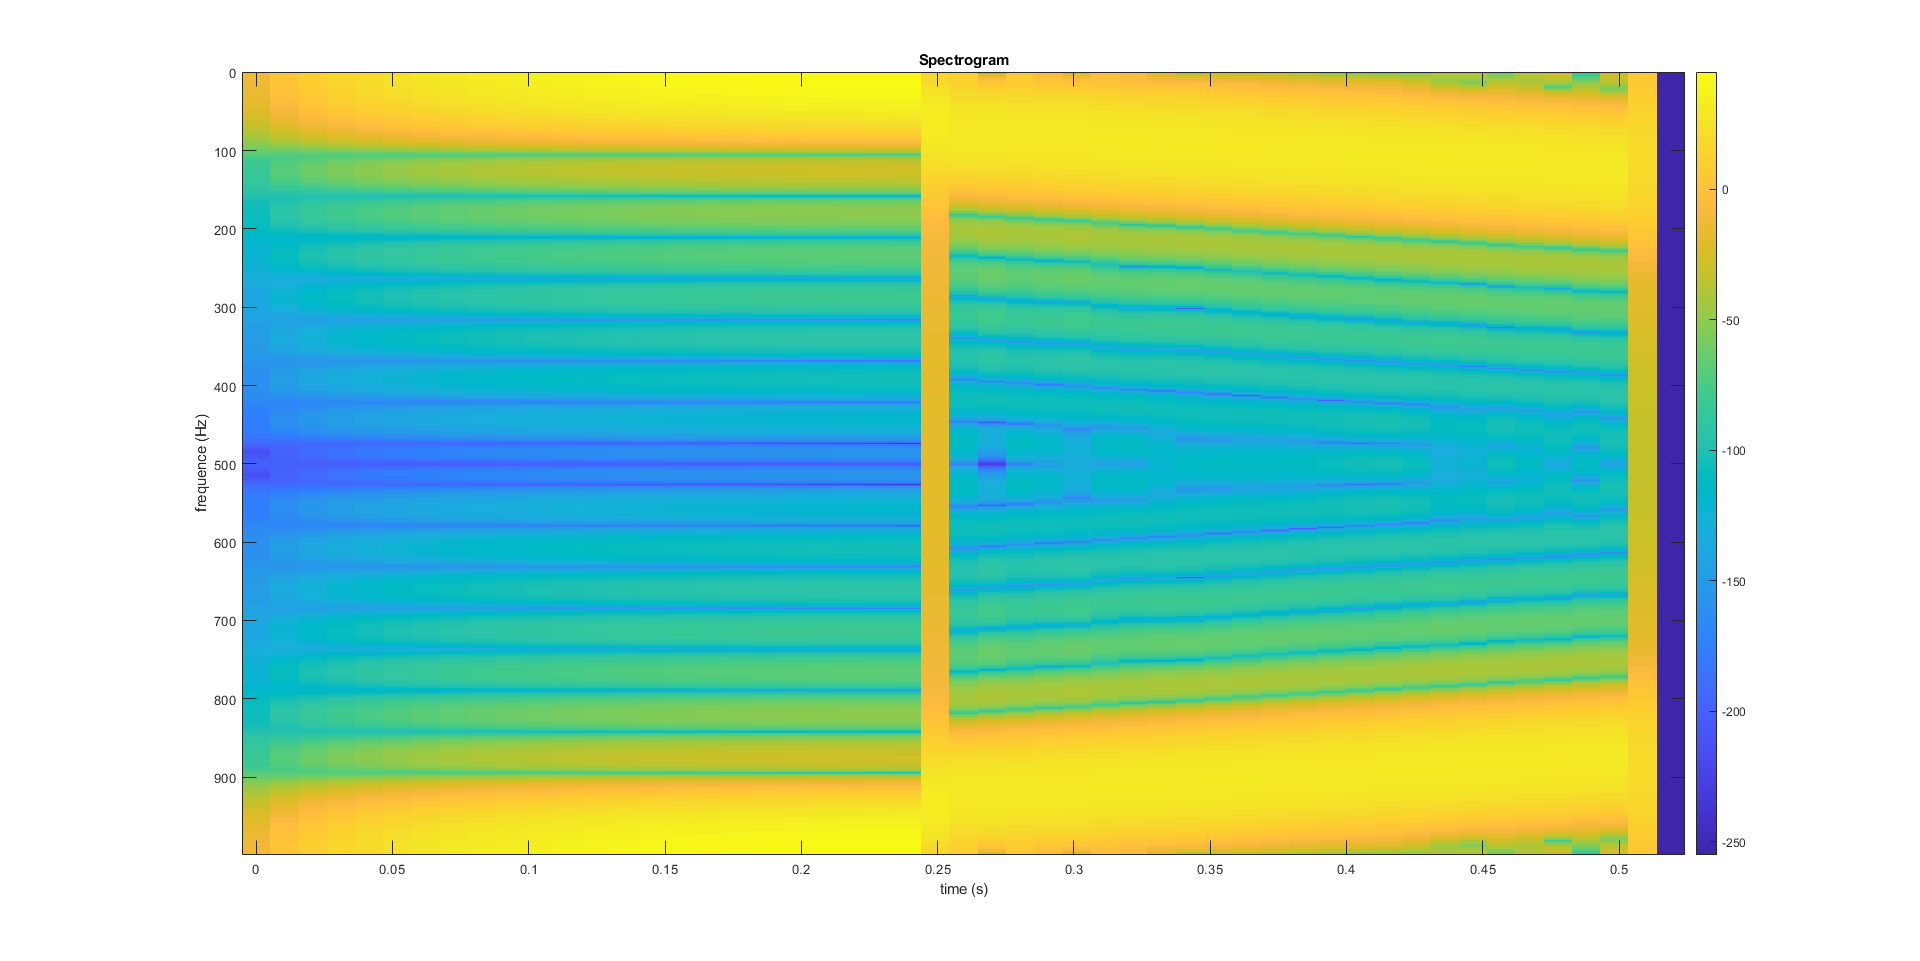
\includegraphics[scale = 0.2]{figure_4_short_window.png}}
\caption{Spectrogram with a short window.}
\end{subfigure}

\end{figure}

This duality between frequency precision and time accuracy can be shown by the example ./src/duality\_time\_frequence.m. In this script the spectrogram of the same signal is plotted using a large window in figure 3 and shorter one in figure 4.

In figure 3, the yellow line is thin compared to the one in figure 3, facilitating to us the reading of frequency value. On the other hand, it’s very difficult to read the transition at 0.25s in comparison with figure 4.

\section{QRS complex Detection}

The QRS complex is going to be detected using the Pan and Tompkins algorithm.The first step of this algorithm eliminates the interference of T and P waves with the QRS complex. A well designed filter is proposed by Pan and Tompkins for this task. Its transfer function is given by :

\begin{equation}
    H(z) = \frac{(1-z^{-6})^{2}}{(1-z^{-1})^{2}}\times\frac{(-1 + 32z^{-16} -32z^{-17} +z^{-32})}{(1-z^{-1})}
\end{equation}

Observing the fact that the R wave is very sharp,the derivative of the ECG signal is going to take big absolute values at the QRS complex.Pan and Tompkins suggests this time a filter with a transfer function equal to :

\begin{equation}
    H(z) = \frac{1}{8T_s}\times(-z^{-2} - 2z^{-1} +2z +z^{2})
\end{equation}

As a consequence, if a well chosen window is used for moving window integration,the result will be a signal which takes big values for every QRS complex.

In order to enhance the QRS complex domain, a thresholding operation is applied with a threshold equal to the mean of ECG signal after integration.

At this point, it’s certain that the computed maximum for every QRS domain corresponds to the unique pick called R.

Once the R pick is detected, Q and S are detected by searching consecutively the first minimum on the left and the first minimum on the right.

All those steps are applied to an ECG signal. The result at every step are plotted in figure 5.


\begin{figure}[htbp]

\centerline{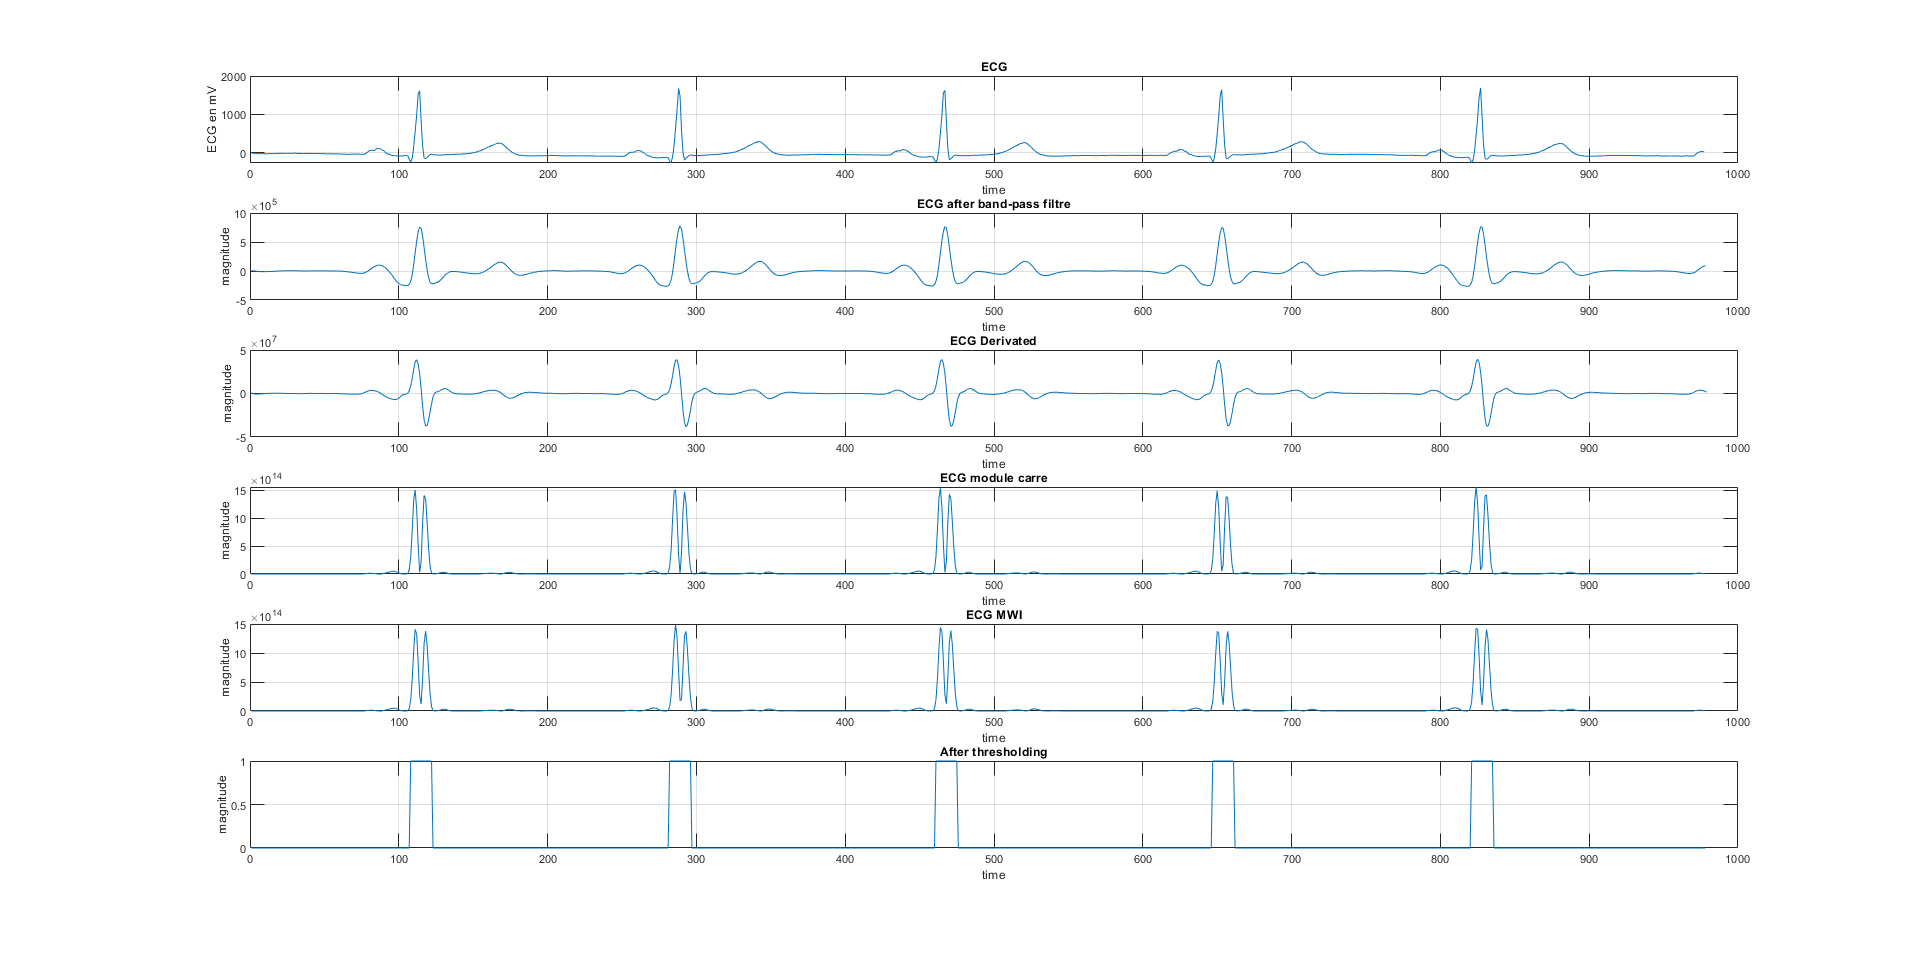
\includegraphics[scale = 0.4]{figure_5.png}}
\caption{ECG signal in each step.}

\end{figure}

\begin{tabular}{ |p{5cm}|p{5cm}|p{5cm}|  }
\hline
\multicolumn{3}{|c|}{Used filters analyse} \\
\hline
band-pass filter &  high-pass filter & five-point differentiation filter\\
\hline
Nature : band-pass & Nature : high-pass & Nature : differentiation\\
Type : Infinite Impulse Response & Type : Infinite Impulse Response & Type : Finite Impulse Response \\
Causal : Yes & Causal : Yes   & Causal : No \\
Group delay : 5 samples &Group delay : 16.49 samples & Group delay : 0 \\
Linear phase : Yes & Linear phase : Yes & Linear phase : Yes\\
\hline
\end{tabular}

\newpage

\section{P and T wave detection}
\subsection{About P and T waves}

Generally, P and T waves in an  ECG (electrocardiogram) signal are lower in amplitude compared to a QRS complex, and, they are contaminated with noise from various sources. These factors make the detection of P and T waves within an ECG a challenging task. Unlike a P wave, T waves are slightly asymmetrical,  the peak of the wave is a little closer to its end than to its beginning.
\subsection{P and T waves detection method}
T waves are considered to be the highest peak between the first R peak and 0.7 times the R-R interval. While P waves have the highest peak in the remaining of the interval, as shown in the figures below.

\begin{figure}[htbp]

\centerline{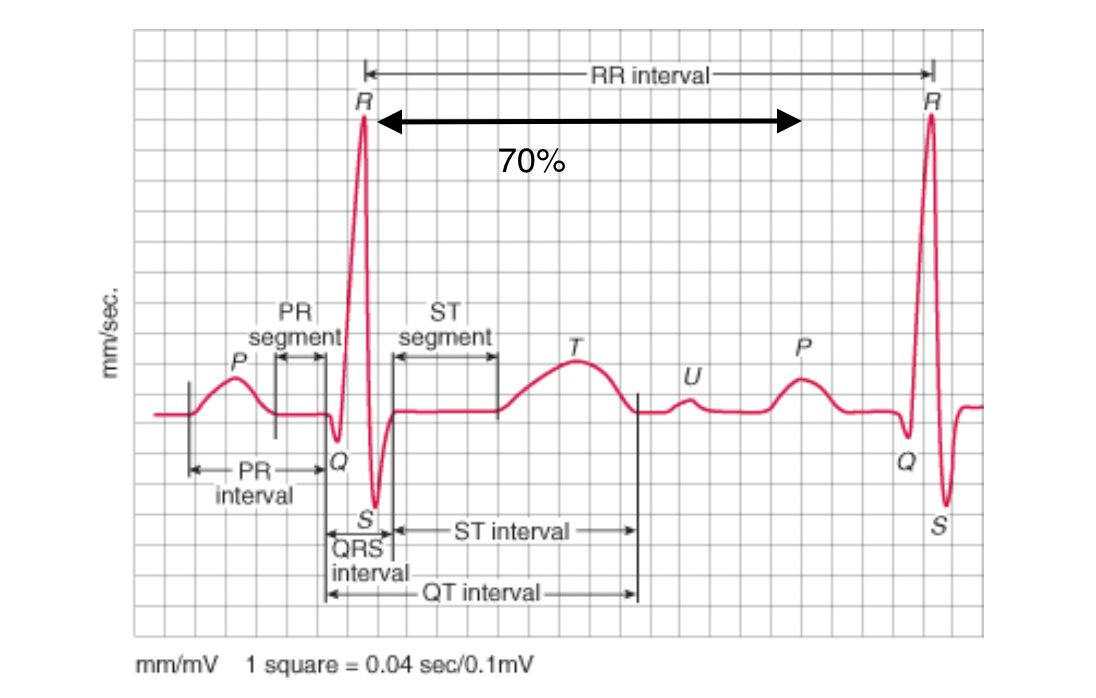
\includegraphics[scale=0.5]{T_70.png}}
\caption{Highest peak on 70\% of R-R interval.}

\end{figure}

\begin{figure}[htbp]

\centerline{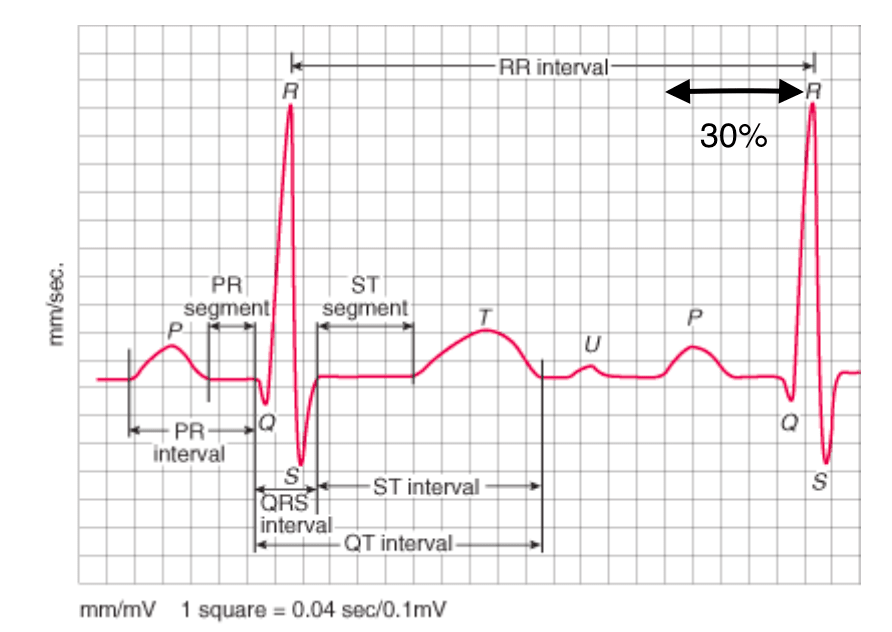
\includegraphics[scale=0.5]{P_30_30.png}}
\caption{Highest peak on the remaining 30\% of R-R interval.}

\end{figure}


In order to detect P and T waves, two filters are used:
 \begin{equation}
     G_1(z) = 1 -z^{-6}
 \end{equation}
 
 and
 
 \begin{equation}
     G_2(z) = \frac{1-z^{-8}}{1-z^{-1}}
 \end{equation}
 
 The first filter \textit{$G_1(z)$} is a differentiator, it allows the detection of maximum, minimum, as well as null values. This is achieved by determining where the signal, after applying the differentiator \textit{$G_1(z)$}, crosses the level 0.
 
 The Algorithm functions as follows: The R-R interval is divided into two parts, a part containing 70\% of the R-R interval, in which T waves are located; and another part containing the remaining 30\% of the R-R interval, in which P waves are located. In each part, the locations in which the signal (after crossing both filers (\textit{$G_1(z)$} and (\textit{$G_2(z)$}) crossed the level 0 were determined. As mentioned before, these locations correspond to either a maximum, minimum, or null values in the original ECG signal. Therefore, the locations that provide a maximum value, are where P and T waves are located.
 
 The figures below illustrate the locations of P and T waves in the original signal,as well as their location after each filter.
 


\begin{figure}[H]
\centerline{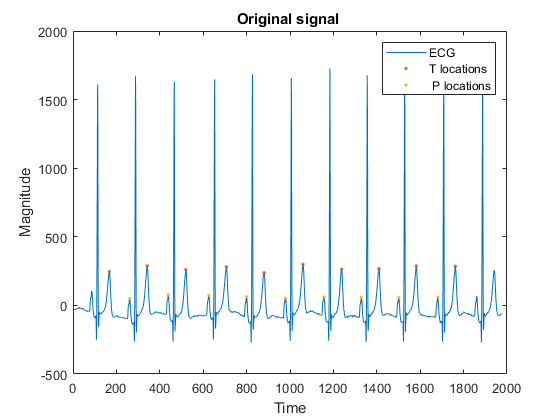
\includegraphics[scale=0.5]{ori_sig.png}}
\caption{Original ECG with locations of P and T waves}
\end{figure}

\begin{figure}[H]
\centerline{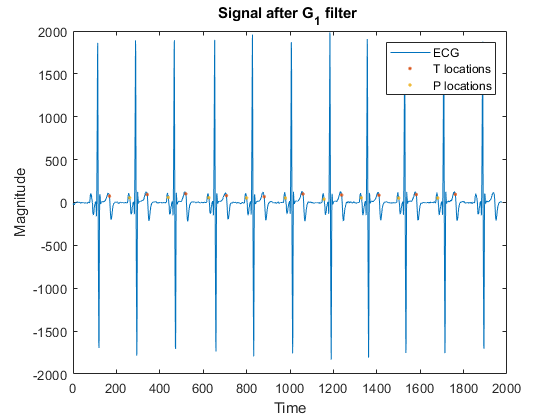
\includegraphics[scale=0.5]{sig_G1.png}}
\caption{ECG after undergoing first filter}
\end{figure}

\begin{figure}[H]
\centerline{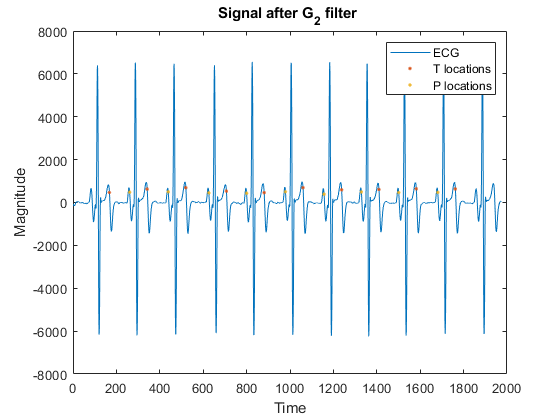
\includegraphics[scale=0.5]{sig_G2.png}}
\caption{ECG after undergoing second filter}
\end{figure}
 

\section{Tachycardia/Bradycardia}

\subsection{Bradycardia}

Bradycardia is defined as a heart rate (HR) of less than 50 or 60 bpm (beats per minute), compared to a normal heart rate of 60 to 100 bpm. A slow heart rate is in general a sign of good health and fitness. However, a heart rate that is too slow (\textit{ie} Bradycardia ), is a sign of a problem with the heart's electrical system. It means that the heart's natural pacemaker isn't working right or that the electrical pathways of the heart are disrupted. The heart beat can be so slow that it can't pump enough blood for the body. Which could be life-threatening if left untreated.

\subsection{Tachycardia}
 
Tachycardia is defined as a heart rate (HR) of over 100 bpm (beats per minute). With atrial or supraventricular tachycardia, electrical signals in the heart’s upper chambers fire abnormally. This interferes with the heart’s natural pacemaker, and causes abnormal heart rates. This rapid heartbeat keeps the heart’s chambers from filling completely between contractions, which compromises blood flow to the rest of the body. 

\subsection{Detecting cardiac rhythm anomalies: Tachycardia and Bradycardia}

An algorithm that calculates the heart rate of a patient, would make it possible to detect cardiac rhythm anomalies. The R waves mark the moment in which the heart beats. Therefore, the duration between consecutive R peaks would help determine the heart rate.
The value calculated is:

\begin{equation}
    \overline{\Delta} = \frac{1}{N}\times\sum_{n=0}^{N-1}\Delta_n
\end{equation}

$\overline{\Delta}$ is the mean of R-R intervals duration. It's value was converted to bpm (beats per minute) by multiplying with \textit{$F_s$} and by 60.


\section{Other pathologies}

\subsection{Ectopic beats}
An ectopic heartbeat is when the heart either skips a beat, or adds an extra beat. They are also called premature heartbeats. Ectopic heartbeats are usually not a cause for concern, and they may occur for no known reason. Despite the skipped or added beat, the heart  functions normally.

\subsection{Detecting ectopic beats}

Detecting premature heartbeats, comes down to detecting irregularities in R-R intervals, since, as mentioned earlier (\textit{section 5.3}), R peaks characterize the moment in which the heart beats.

The algorithm devised, calculated the length of different R-R intervals,and chose their maximum value, since an ectopic beat is placed either to close or too far from a regular beat, either a maximum or a minimum value would have been appropriate.
By calculating the same value for normal patients, a threshold $\epsilon$ was determined as $\epsilon = 1$.
This value (\textit{\textbf{max}}) was calculated for different patients, and compared with $\epsilon$.
The results were consistent, \textit{\textbf{max}} was Superior to $\epsilon$ in patients with ectopic beats, and inferior or equal on other cases.

\section{Fibrillation}

\subsection{Atrial fibrillation}


Atrial fibrillation is characterized by a strong heart rhythm irregularity until the point of considering it as white noise. The main property of a white noise is that its autocorrelation function is null except in zero. That is why autocorrelation function of the studied ECG is estimated with the formula :

\begin{equation}
    \hat{\gamma_k} = \frac{1}{N-k-1}\times\sum_{n=0}^{N-k-1} (\Delta_{n+k} - \overline{\Delta})(\Delta_{n} - \overline{\Delta})
\end{equation}

\begin{figure}
\centerline{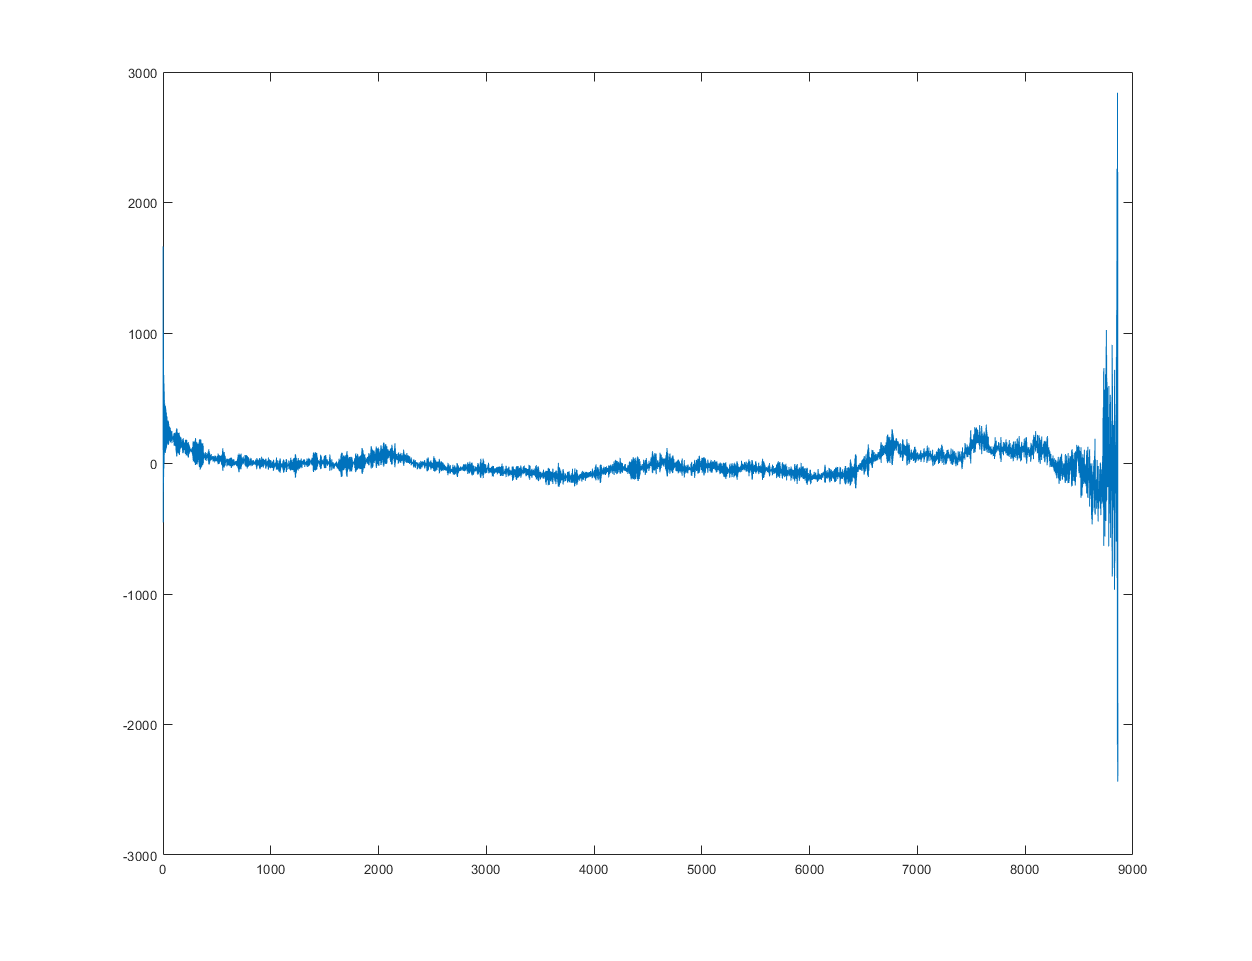
\includegraphics[scale=0.4]{figure_6_edge_effect.png}}
\caption{Edge effect.}
\end{figure}

Figure 11 is an example of an estimated autocorrelation function. At the right of the figure, big random values are remarked because, in this area,the autocorrelation is estimated using a small number of samples so the mean is not representative enough. For that reason, the studied domain of the autocorrelation function is not going to include the values at the right edge.

The heart rhythm is going to be considered as a white noise if 40\% of its autocorrelation function at zero is still a maximum of the autocorrelation function.

\subsection{Ventricular fibrillation}

Ventricular fibrillation, or V-fib, is considered the most serious cardiac rhythm disturbance.
Disordered electrical activity causes the heart’s lower chambers (ventricles) to quiver, or fibrillate, instead of contracting (or beating) normally. This prohibits the heart from pumping blood. Thus leading to collapse and cardiac arrest

\subsection{Detecting ventricular fibrillation}

Two main properties are used to detect Ventricular fibrillation: The similarity between the ECG (electrocardiogram) of the patient and the pure sine; as well as a rapid heart rate between 240 and 600 bpm (beats per minute).
The similarity between Ventricular fibrillation ECG and the pure sine function was detected by resorting to the Fourier transform. Plotting the two Fourier transforms, illustrates the similarity between them, as shown below.
\textbf{N.B: FT = Fourier transform}

\newpage

\begin{figure}
\centerline{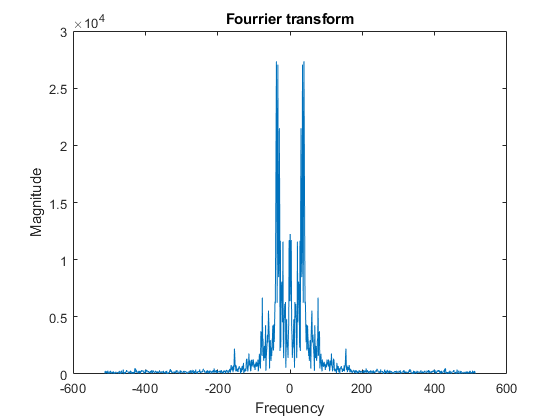
\includegraphics[scale=0.6]{Fourrier_VF.png}}
\caption{TF of ECG}
\end{figure}
\begin{figure}
\centerline{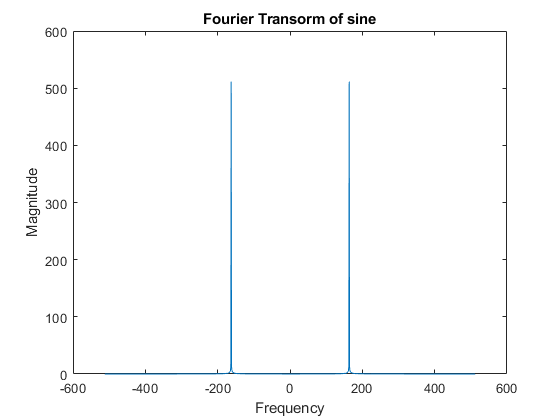
\includegraphics[scale=0.6]{sin_fou.png}}
\caption{TF of sine}
\end{figure}

\newpage

The FT are similar, with two important peaks at symmetric values of frequency. In order to detect the two peaks,  a threshold was applied to the FT,in order to calculate the number of values superior to $0.8\times\textit{n}$; where \textit{n} is the maximum value of the FT. An ECG with a ventricular fibrillation generally has a low number of values above  $0.8\times\textit{n}$, compared to other ECGs, combining this with the condition of a heart rate between 240 and 600 bpm, a case of ventricular fibrillation can be determined




\section{Conclusion}
This report has discussed the implementation of algorithms used to detect PQRST waves and automatic heart pathology identification. Besides that, it has introduced the utility of spectrograms as well as their limitations. The results obtained were satisfying. However, we really wished to develop a graphic user interface to make our work valuable but we could not because we did not have enough time.

\newpgae

\begin{thebibliography}{2} 
   \bibitem[1]{cle} P and T waves https://pubmed.ncbi.nlm.nih.gov/29484531/
   \bibitem[2]{cle} Bradycardia   https://www.uofmhealth.org/health-library/aa107571
   \bibitem[3]{cle} tachy https://pubmed.ncbi.nlm.nih.gov/29484531/
   \bibitem[4]{cle} ectopic https://www.medicalnewstoday.com/articles/323202#what-is-an-ectopic-heartbeat
   \bibitem[5]{cle} Ventr fibr https://www.heart.org/en/health-topics/arrhythmia/about-arrhythmia/ventricular-fibrillation
   
\end{thebibliography} 

\end{document}


